\section{Question and answer}\label{sec:question}

\textbf{Question.} How much of the Hurst exponent of a mountain flight comes from the geometry of the crests alone?
The exponent $H$ is half the log-log slope of the mean squared displacement (MSD). We measure $\Hgeo$ of a ball that runs at
constant speed along the crests of the French Alps and the Pyrenees, and compare it with that of paraglider flights, in
time ($\Hdyn$) and along their route ($\Hroute$).

\smallskip
\noindent\textbf{Answer.}
\begin{itemize}[nosep,leftmargin=1.5em]
  \item The crests are close to straight and bend more as the scale grows: the local slope of the MSD falls
        with the scale and has no plateau (Figure~\ref{fig:routealpha}, Section~\ref{sec:results}).
  \item Along their route the flights are about as straight as the crests: $\Hroute$ is just below $\Hgeo$ in both
        massifs (Table~\ref{tab:flh}, Section~\ref{sec:flights}).
  \item In time the exponent is lower ($\Hdyn$), because the flights leave the ballistic regime within seconds
        (Section~\ref{sec:flights}).
  \item Box counting, which uses no MSD, gives $D=1/H$ within 0.01 for the crests and the routes. Between 1 and 10~km crests
        and routes share $D$ within the spread between two estimators (about 0.02); below 1~km the route is rougher
        (Section~\ref{sec:dimension}).
\end{itemize}

\begin{figure}
\centering
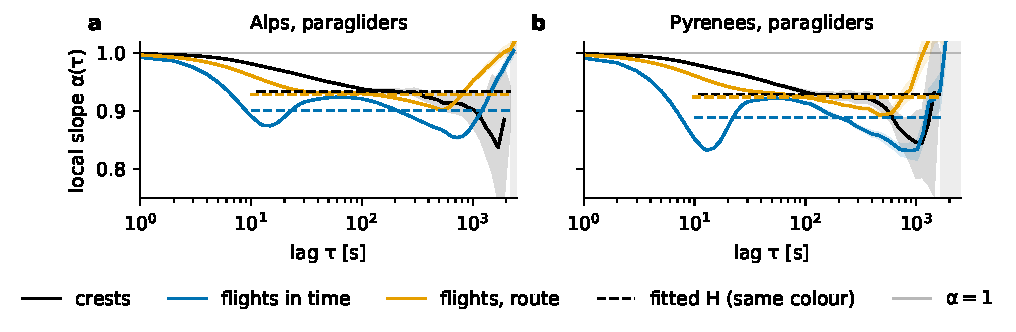
\includegraphics[width=\textwidth]{figures/route_alpha}
\caption{The route of the flights follows the crests, and the flights in time fall below both. Local slope of the MSD, $\alpha(\tau)$, against the lag
$\tau$ for the Alps (\textbf{a}) and the Pyrenees (\textbf{b}) paragliders. Crests and route are in arc length, read as lags at the mean glide speed. Dashed lines: $H$ of the
rule of Section~\ref{sec:flcurves} over the lags of the fit. Bands: 95\% bootstrap intervals; grey zone: beyond the last lag of the fit.}
\label{fig:routealpha}
\end{figure}

\begin{table}[H]
\centering
\caption{The route is as straight as the crests; in time the exponent is lower. $H$ by the rule of Section~\ref{sec:flcurves}, with 95\% bootstrap intervals.}
\label{tab:flh}
\small
\begin{tabular}{lll}
\toprule
curve & Alps, paragliders & Pyrenees, paragliders \\
\midrule
number of flights & 23320 & 2140 \\
crests, $\Hgeo$ & 0.934 (0.930--0.940) & 0.929 (0.926--0.933) \\
route of the flights, $\Hroute$ & 0.929 (0.929--0.930) & 0.925 (0.923--0.926) \\
flights in time, $\Hdyn$ & 0.901 (0.901--0.902) & 0.890 (0.888--0.892) \\
\bottomrule
\end{tabular}

\end{table}
